%%%% rapport.tex

\documentclass{article}
\pdfpagewidth=8.5in
\pdfpageheight=11in
\usepackage{ijcai19}

\usepackage{times}
\usepackage{soul}
\usepackage{url}
\usepackage[hidelinks]{hyperref}
\usepackage[utf8]{inputenc}
\usepackage[small]{caption}
\usepackage{graphicx}
\usepackage{amsmath}
\usepackage{booktabs}
\usepackage{algorithm}
\usepackage{algorithmic}
\urlstyle{same}

\title{Exploration d'un Resnet pour la classification d'images}

\author{
Nicolas Dépelteau
\and
Dung Nguyen
\affiliations{}
Polytechnique Montréal
\emails{}
nicolas.deplteau@polymtl.ca,
thi-ngoc-dung.nguyen@polymtl.ca
}

\begin{document}

\maketitle

\begin{abstract}
    Dans ce rapport écrit pour notre projet dans le cadre du cours INF8225,
    nous présentons les bénéfices de l'utilisation
    d'un Resnet dans le cadre de la classification d'images. Nous avons également comparé les
    résultats de notre Resnet avec ceux d'un réseau de neurones convolutif simple. 
\end{abstract}

\section{Introduction}

Plusieurs travaux ont été proposés pour améliorer les performances des réseaux de neurones profonds pour la classification d'images.
Parmi ces travaux, on peut citer l'article ``Very Deep Convolutional Networks for Large-Scale Image Recognition'' proposé par Karen
Simonyan et Andrew Zisserman en 2015~\cite{simonyan2015deep}, qui proposait des réseaux VGG ayant jusqu'à 19 couches de convolution pour extraire des
caractéristiques visuelles à partir des images.
Cependant, malgré des performances de classification impressionnantes, ces réseaux de neurones profonds ont été confrontés à un
problème de dégradation des performances avec l'augmentation de la profondeur.
C'est dans ce contexte que l'article ``Deep Residual Learning for Image Recognition'' proposé par Kaiming He, Xiangyu Zhang,
Shaoqing Ren et Jian Sun en 2016~\cite{resnet}, a introduit les connexions résiduelles pour permettre un apprentissage en profondeur plus efficace
et surmonter ce problème de dégradation.
Dans ce texte nous allons présenter les réseaux de neurones convolutifs et les connexions résiduelles ainsi que nos expériences
sur ceux-ci.

\section{Les réseaux convolutifs (CNN)}
Un réseau convolutif est un réseau dans lequel les neurones sont organisés en couches.
Chaque couche est composée de plusieurs neurones. Chaque neurone est connecté à tous les neurones de la couche précédente.
Chaque connexion est associée à un poids. Lorsque le réseau est activé, chaque neurone calcule une somme
pondérée des valeurs de sortie des neurones de la couche précédente.
Cette opération est une convolution dans le cas d'un réseau convolutif.
Cette somme est ensuite passée à une fonction d'activation.
La fonction d'activation est utilisée pour introduire une non-linéarité dans le réseau.
La fonction d'activation la plus utilisée est la fonction ReLU.\@
La fonction ReLU est définie comme suit:
\begin{equation}
    f(x) = \max(0, x)
\end{equation}

\subsection{Convolution}
L'opération de convolution est une opération mathématique qui est utilisée pour extraire des caractéristiques d'une image.
L'opération de convolution est définie comme suit:
\begin{equation}
    S(i, j) = (I * K)(i, j) = \sum_{m} \sum_{n} I(m, n)K(i - m, j - n)
\end{equation}
où $I$ est l'image d'entrée, $K$ est le noyau de convolution et $S$ est l'image de sortie.
Le noyau de convolution est une matrice de taille $m \times n$.
L'image de sortie est une image de taille $m \times n$.
L'image de sortie est calculée en faisant glisser le noyau de convolution sur l'image d'entrée.


\subsection{Regroupement (Pooling)}
Le regroupement est une opération qui est utilisée pour réduire la taille de la carte des caractéristiques.
Le regroupement est effectué en faisant glisser une fenêtre sur la carte des caractéristiques.
La valeur de sortie de la fenêtre est la valeur maximale de la fenêtre dans le cas du ``max pooling''.
Toutefois il existe aussi d'autres types de regroupement comme le ``average pooling''.
Le regroupement par la moyenne est une opération qui est similaire au ``max pooling''.
La valeur de sortie de la fenêtre est la moyenne des valeurs de la fenêtre.
La taille de la fenêtre est un hyper paramètre du réseau.

\subsection{Le problème du gradient qui disparaît (Vanishing gradient problem)}
Le problème du gradient qui disparaît est un problème qui est présent dans les réseaux profonds.
Ce problème est causé par la fonction d'activation ReLU.\@
La fonction ReLU est définie comme suit:
\begin{equation}
    f(x) = \max(0, x)
\end{equation}
La dérivée de la fonction ReLU est définie comme suit:
\begin{equation}
    f'(x) = \begin{cases}
        1 & \text{si } x > 0 \\
        0 & \text{sinon}
    \end{cases}
\end{equation}

Lorsque la fonction ReLU est utilisée comme fonction d'activation, la dérivée de la fonction d'activation est soit 0 ou 1.
Lorsque la dérivée de la fonction d'activation est 0, le gradient est 0.
Lorsque le gradient est 0, le poids n'est pas mis à jour.
Lorsque le poids n'est pas mis à jour, le réseau ne peut pas apprendre.
C'est pourquoi le problème du gradient qui disparaît est un problème qui empêche les réseaux profonds d'apprendre puisqu'il y a plus
de couche à traverser lors de la propagation par l'arrière. Effectivement, un gradient null à une couche profonde empêche
la mise à jour des poids des couches précédentes. Et cela se produit de plus en plus souvent lorsque la profondeur du réseau augmente.

\subsection{Le problème de dégradation}
Le problème de dégradation est un problème qui est présent dans les réseaux profonds.

\begin{figure}[h]
    \centering
    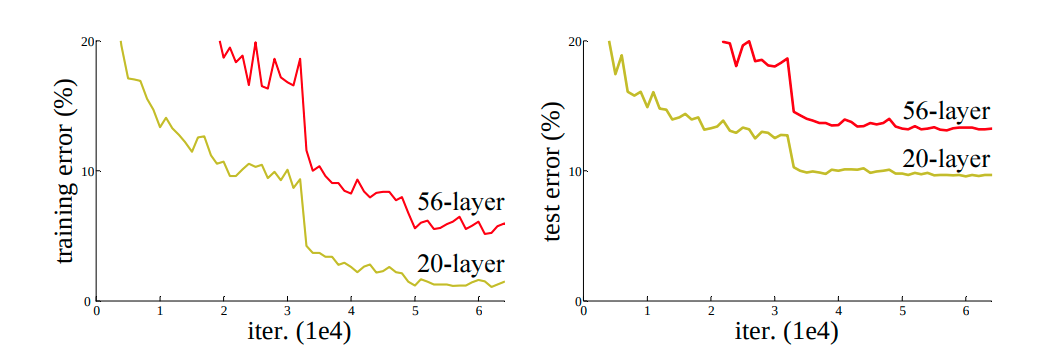
\includegraphics[width=240pt,height=120pt]{./img/degradation}
    \caption{Problème de dégradation: Réseau plus profond avec une plus petite précision}\label{fig: degrad}
\end{figure}

Ce phénomène est contre-intuitif, car on s'attendrait à ce que l'ajout de couches supplémentaires permette au réseau de mieux
capturer les caractéristiques des images et donc d'augmenter ses performances.
Cependant, les auteurs de l'article ``Deep Residual Learning for Image Recognition''~\cite{resnet}
proposent une explication à ce phénomène
en affirmant que les couches profondes ont des difficultés à apprendre des fonctions identité,
c'est-à-dire à conserver l'information non perturbée par la transformation non-linéaire introduite par la couche.
Cette perte d'information a un effet négatif sur les performances du réseau lors de l'ajout de couches supplémentaires.

\section{Resnet}

Pour pallier ce problème, les auteurs proposent d'utiliser des connexions résiduelles pour permettre un apprentissage en
profondeur plus efficace~\cite{resnet}. En effet, au lieu d'apprendre directement la fonction $H(x)$ où $x$ est l'entrée d'une pile
de couche dont la sortie est $H(x)$. Le réseau apprend
plutôt son résidu $F(x) = H(x) - x$. La fonction $F(x)$ est plus facile à apprendre que la fonction $H(x)$, car elle est
plus proche de la fonction identité. La fonction $H(x)$ est alors approximée par la fonction $F(x) + x$.
Le réseau Resnet est composé de plusieurs blocs de convolution, puis d'une couche dense complètement connecté.

\subsection{Connection résiduelle}
La caractéristique la plus particulière de ResNet est que la connection résiduelle est appliquée à l'intérieur de chaque bloc
pour aider le modèle à garder les résidus du passé vers le futur.

\begin{figure}[h]
    \centering
    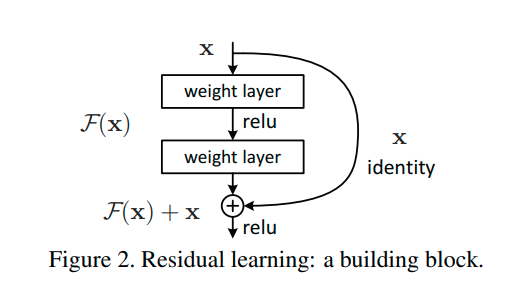
\includegraphics[width=150pt,height=90pt]{./img/skip}
    \caption{Connection résiduel dans un block de ResNet.}\cite{resnet}\label{fig: skip}
\end{figure}

Le bloc de ResNet est composé de deux couches de convolution et d'une couche pour ajuster les dimensions entre $F(x)$ et $x$.
La fonction du bloc i est définie comme suit:

\begin{equation}
    H_i(x) = \sigma(W_{i,2} * \sigma(W_{i,1} * x) + W_{i,3} * x)
\end{equation}

\begin{equation}
    W_{i, 3} =
    \begin{cases}
        I \text{ si les dimensions de x sont identiques à la sortie} \\
        W_{i, 3}\text{ avec un noyau de } 1\times1 \text{ sinon}
    \end{cases}
\end{equation}

où $x$ est l'entrée du bloc, $\sigma$ est la fonction d'activation ReLU, $W_{i,1}$ et $W_{i,2}$ sont les paramètres de la
couche de convolution et $W_{i,3}$ est le paramètre de la couche de la connection résiduelle.


\subsection{normalisation par lots (Batch Normalization)}
ResNet est la première architecture a appliqué normalisation par lots à l'intérieur de chacune des ses couches. La normalisation par lots aide le
modèle à rester stable lors de la descente de gradient et à soutenir la convergence rapide du processus de formation vers
un point optimal.
La normalisation par lots est appliquée sur chaque mini-lot par une normalisation standard d'une gaussienne $N(0,1)$.
On a $B=x_1,x_2,\dots x_m$.
où $m$ indique la taille du mini-lot. Tous les échantillons d'entrée sont redimensionnés comme ci-dessous:
\begin{equation}
    \mu = \frac{1}{m}\sum_{i=1}^{m}x_{i}
\end{equation}

\begin{equation}
    \sigma^{2} = \frac{1}{m}\sum_{i=1}^{m}(x_{i} - \mu)^{2}
\end{equation}

Le nouvel échantillon normalisé est:
\begin{equation}
    \hat{x}_{i} = \frac{x_{i} - \mu}{\sigma}
\end{equation}

\section{Architecture}

L'architecture des modèles que nous avons utilisé est basée sur l'architecture générique de ResNet présentée dans l'article
``Deep Residual Learning for Image Recognition''~\cite{resnet}. Cette architecture est composée de plusieurs blocs de
convolution, puis d'une couche dense complètement connecté. Pour la version avec résiduel, il y a l'opération de l'addition entre
l'entrée du bloc avec ajustement si nécessaire et la sortie, comme montré dans la figure~\ref{fig: res_blocs}.
Il y a également une normalisation par lots après les convolutions.
il y a un dropout avec une probabilité de 0.5.

\begin{figure}[h]
    \centering
    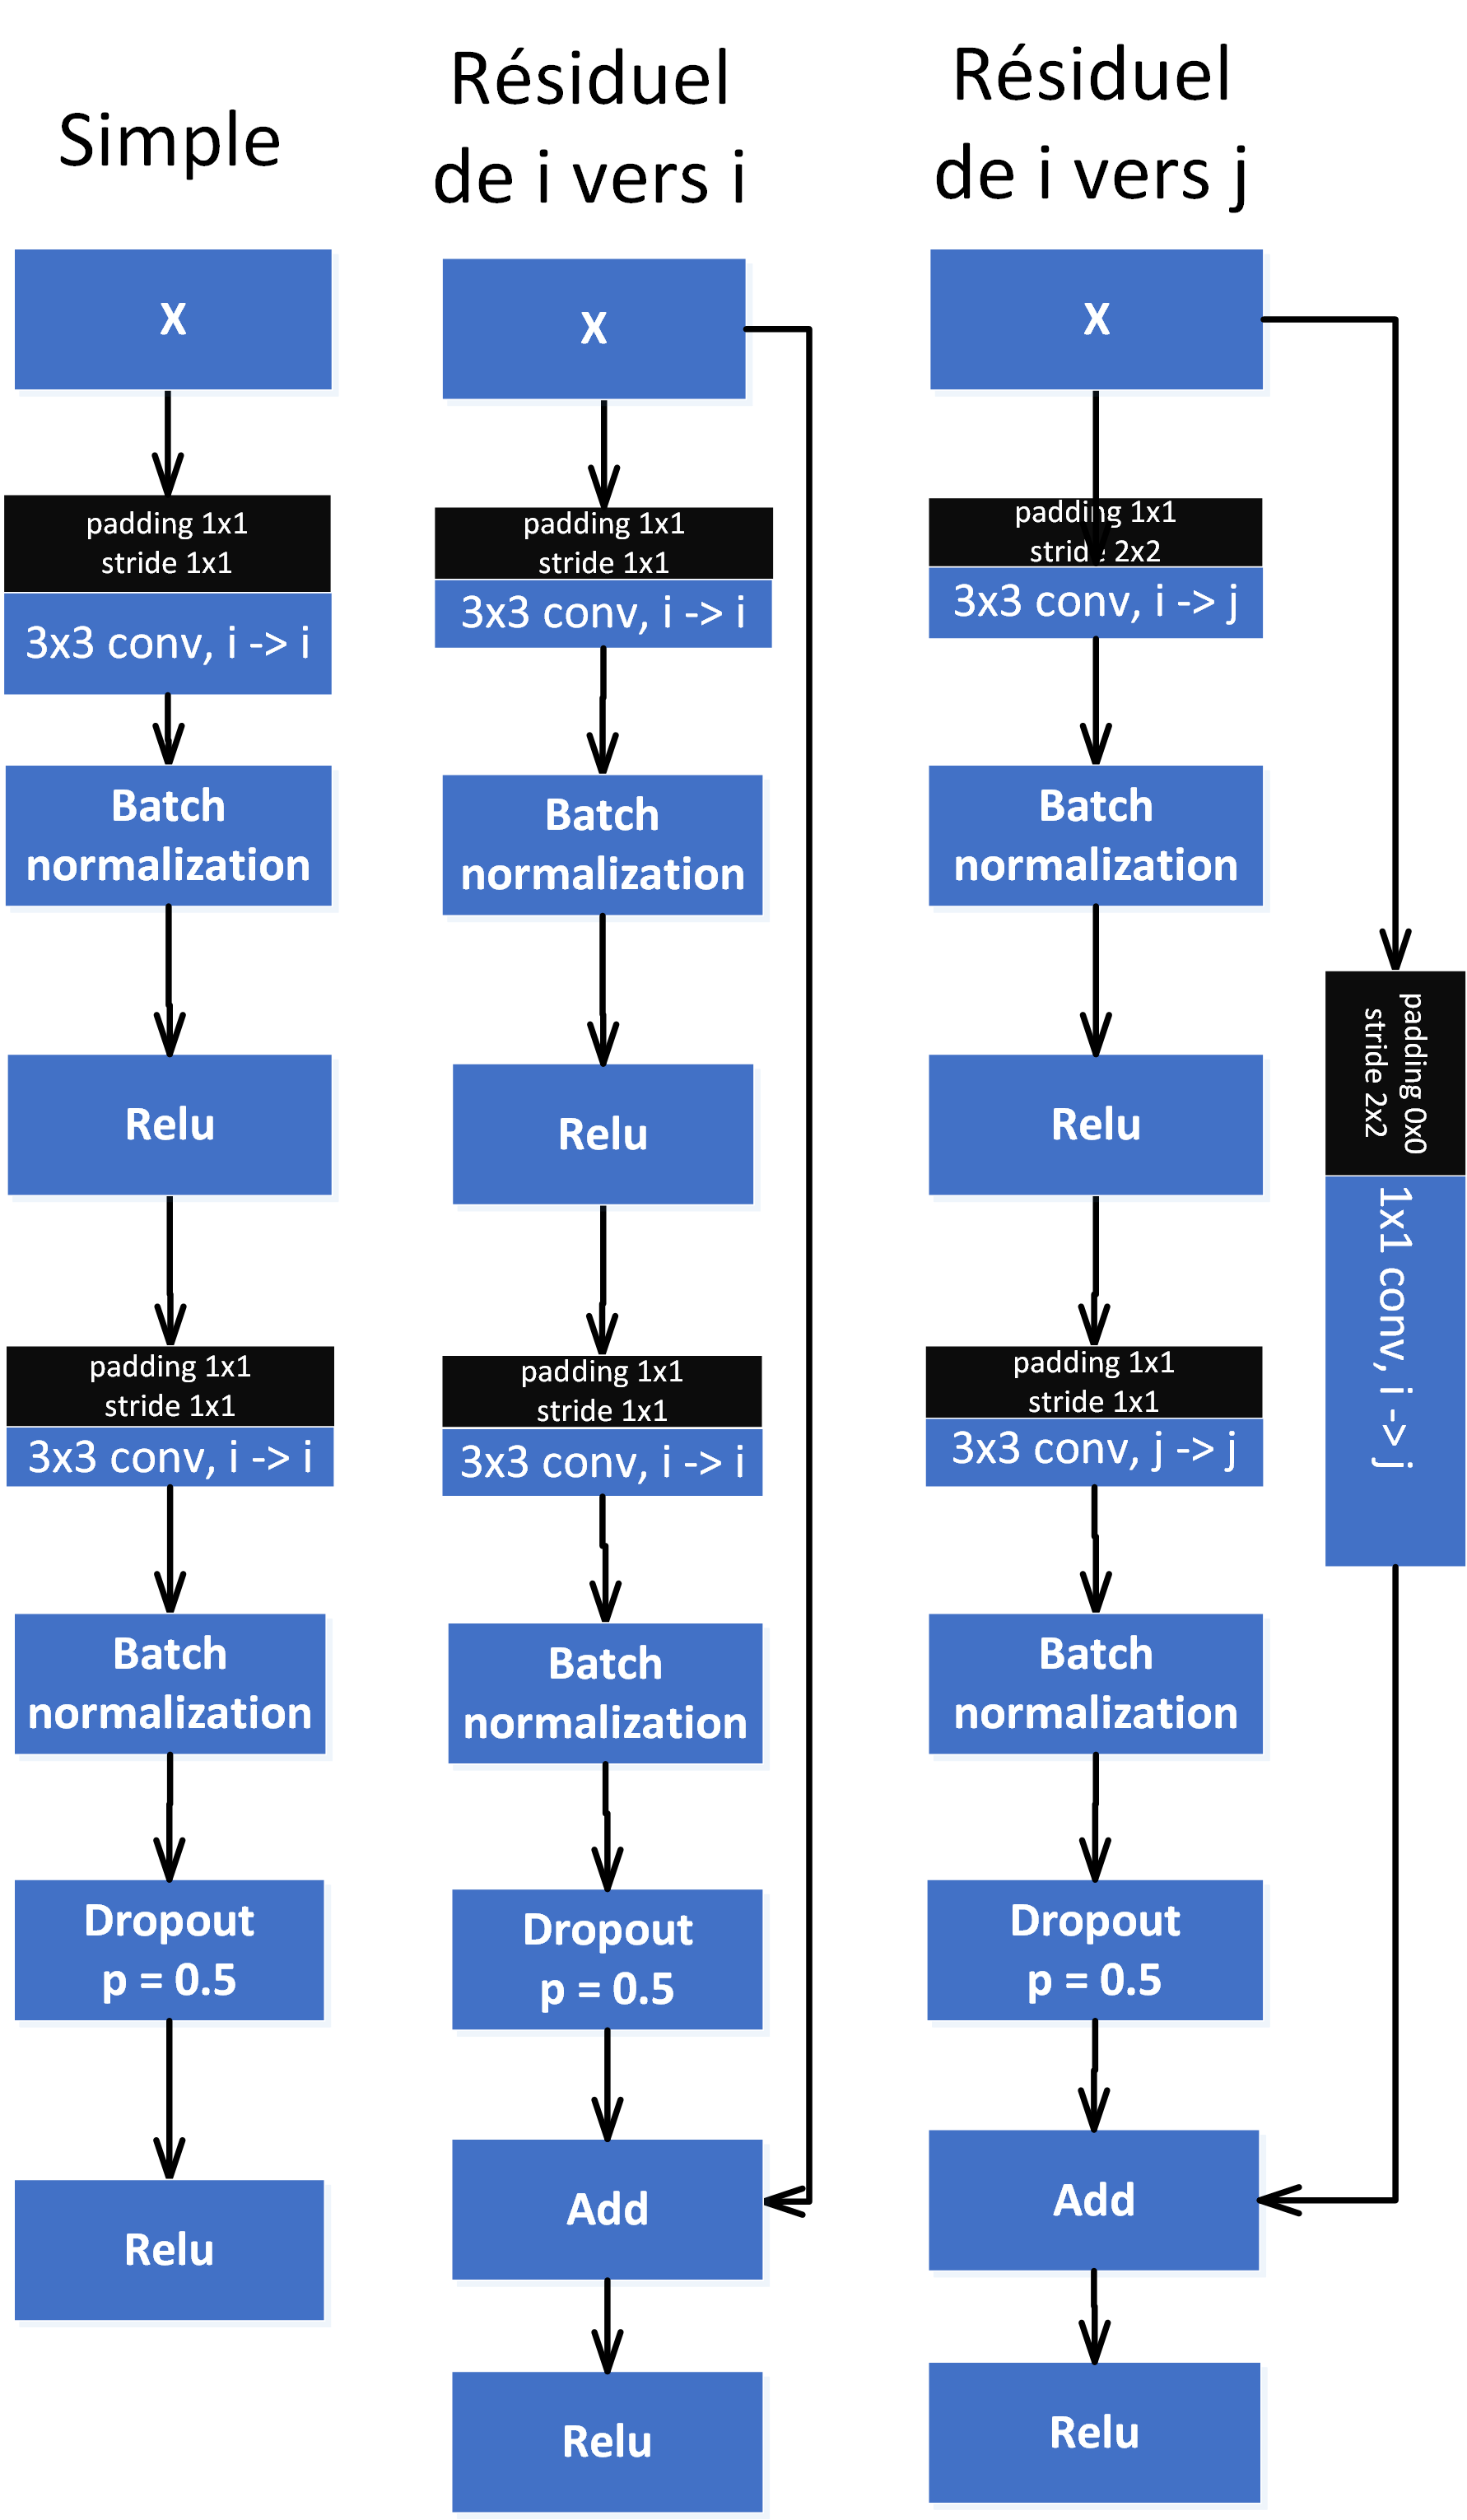
\includegraphics[width=240pt,height=450pt]{./schema/bloc.png}
    \caption{Blocs résiduels}\label{fig: res_blocs}
\end{figure}


\begin{figure}[h]
    \centering
    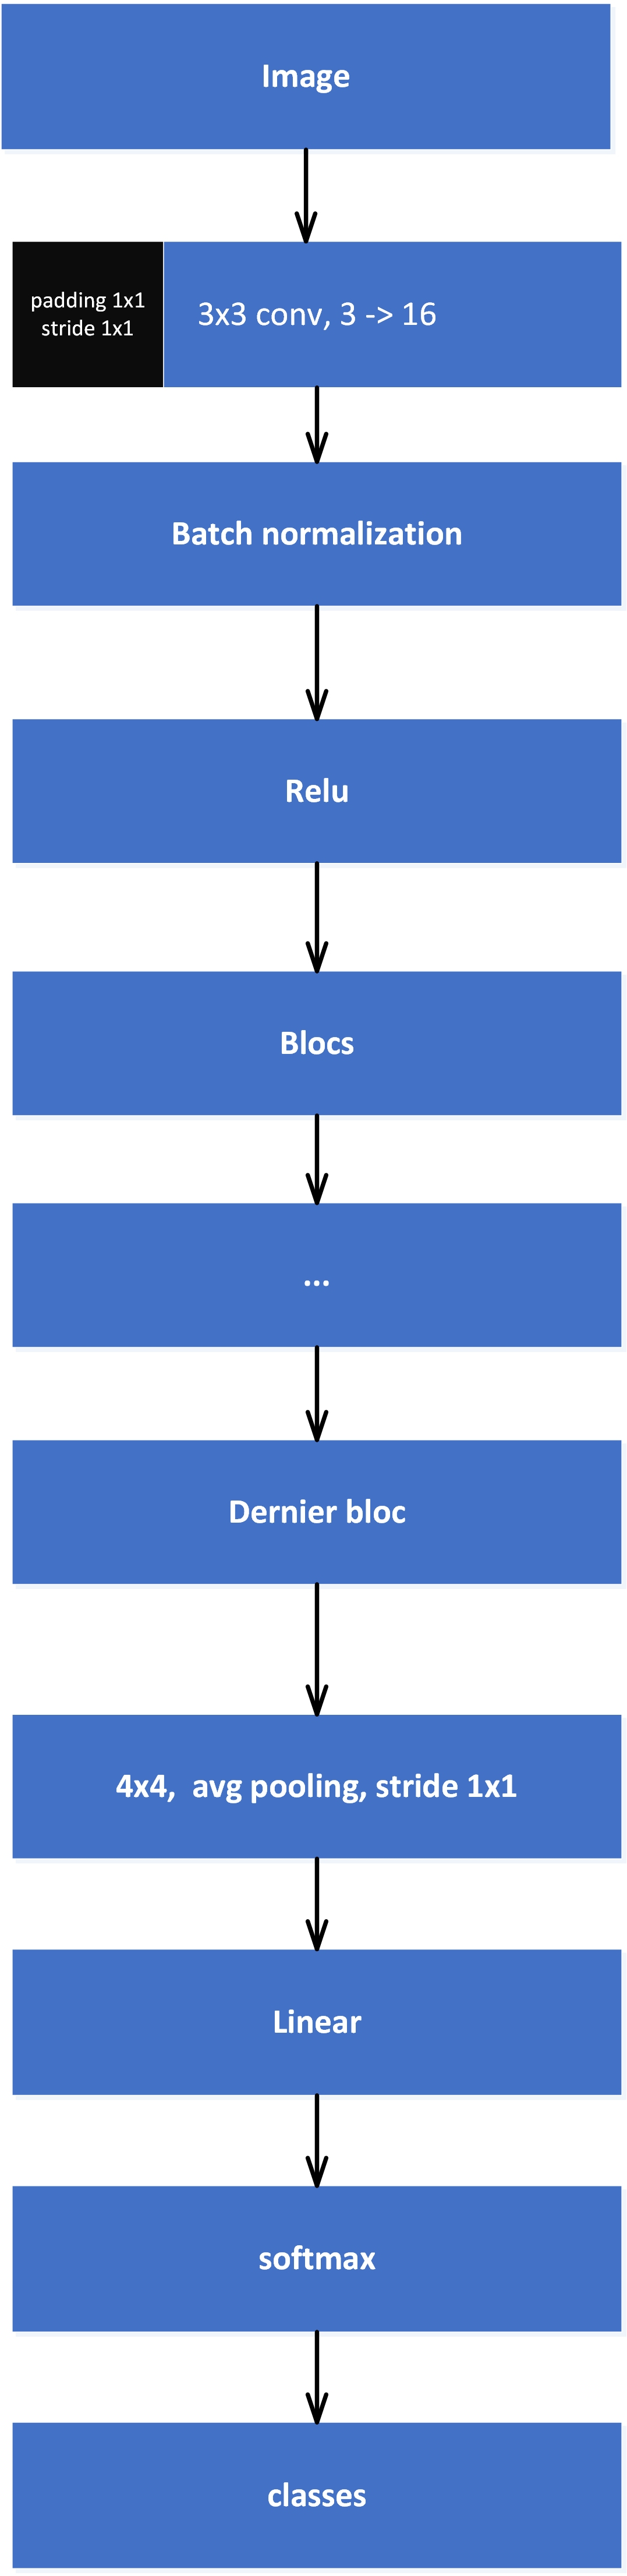
\includegraphics[width=120pt,height=370pt]{./schema/net.png}
    \caption{Architecture générique du model}\label{fig: net}
\end{figure}

Le tableau~\ref{tab:resnet} montre les différentes architectures que nous avons utilisées. Les architectures sont
définies par leur nombre de blocs résiduels. Par exemple, la plus petite architecture avec seulement 8 couches contient
des blocs résiduels respectif de 16 à 32, 32 à 64 et 64 à 128. Il ne faut pas oublié que ces blocs sont insérés dans l'architecture
générique de ResNet présentée dans la figure~\ref{fig: net}.

\begin{table}[H]
\centering
\begin{tabular}{llllll}
\hline
Blocs résiduels & 8 & 14 & 18 & 34 & 50 \\
\hline
16 $\rightarrow $ 16 & - & 1 & 1 & 3 & 6 \\
16 $\rightarrow $ 32 & 1 & 1 & 1 & 1 & 1 \\
32 $\rightarrow $ 32 & - & 1 & 1 & 3 & 5 \\
32 $\rightarrow $ 64 & 1 & 1 & 1 & 1 & 1 \\
64 $\rightarrow $ 64 & - & - & 1 & 5 & 5 \\
64 $\rightarrow $ 128 & 1 & 1 & 1 & 1 & 1 \\
128$\rightarrow $ 128 & - & 1 & 1 & 2 & 5 \\
\hline
\end{tabular}
\caption{Nombre de blocs résiduels pour chacune des architectures ayant un nombre de couche différent}\label{tab:resnet}
\end{table}

\section{Expérimentation}

Dans ce rapport, nous allons explorer la performance de cinq modèles de ResNet: ResNet-8, ResNet-14, ResNet-18, ResNet-34 et ResNet-50.
Nous avons entraîné les cinq modèles de ResNet sur un jeu de données d'images, en utilisant la bibliothèque PyTorch.

\subsection{Le jeu de données}

Le jeu de données utilisé est le jeu de données CIFAR-10, qui contient 50 000 images d'entraînement et 10 000 images
de test. Les images sont de taille 32$\times$32 pixels et appartiennent à 10 classes différentes. Les classes sont:
avion, automobile, oiseau, chat, cerf, chien, grenouille, cheval, bateau et camion. Les images sont en couleur,
chaque pixel est représenté par trois valeurs de 0 à 255, une pour chaque canal de couleur soit le rouge, le vert et le bleu.

\subsection{Les hyper paramètres}

Nous avons utilisé une fonction de perte de type ``cross-entropy'' et un optimiseur de type ``Adam'' pour entraîner les modèles.
Les modèles ont été entraînés pendant 10 époques.

\subsection{Les résultats}

Les résultats de l'expérimentation sont présentés dans la graphique 4.

\begin{figure}[h]
    \centering
    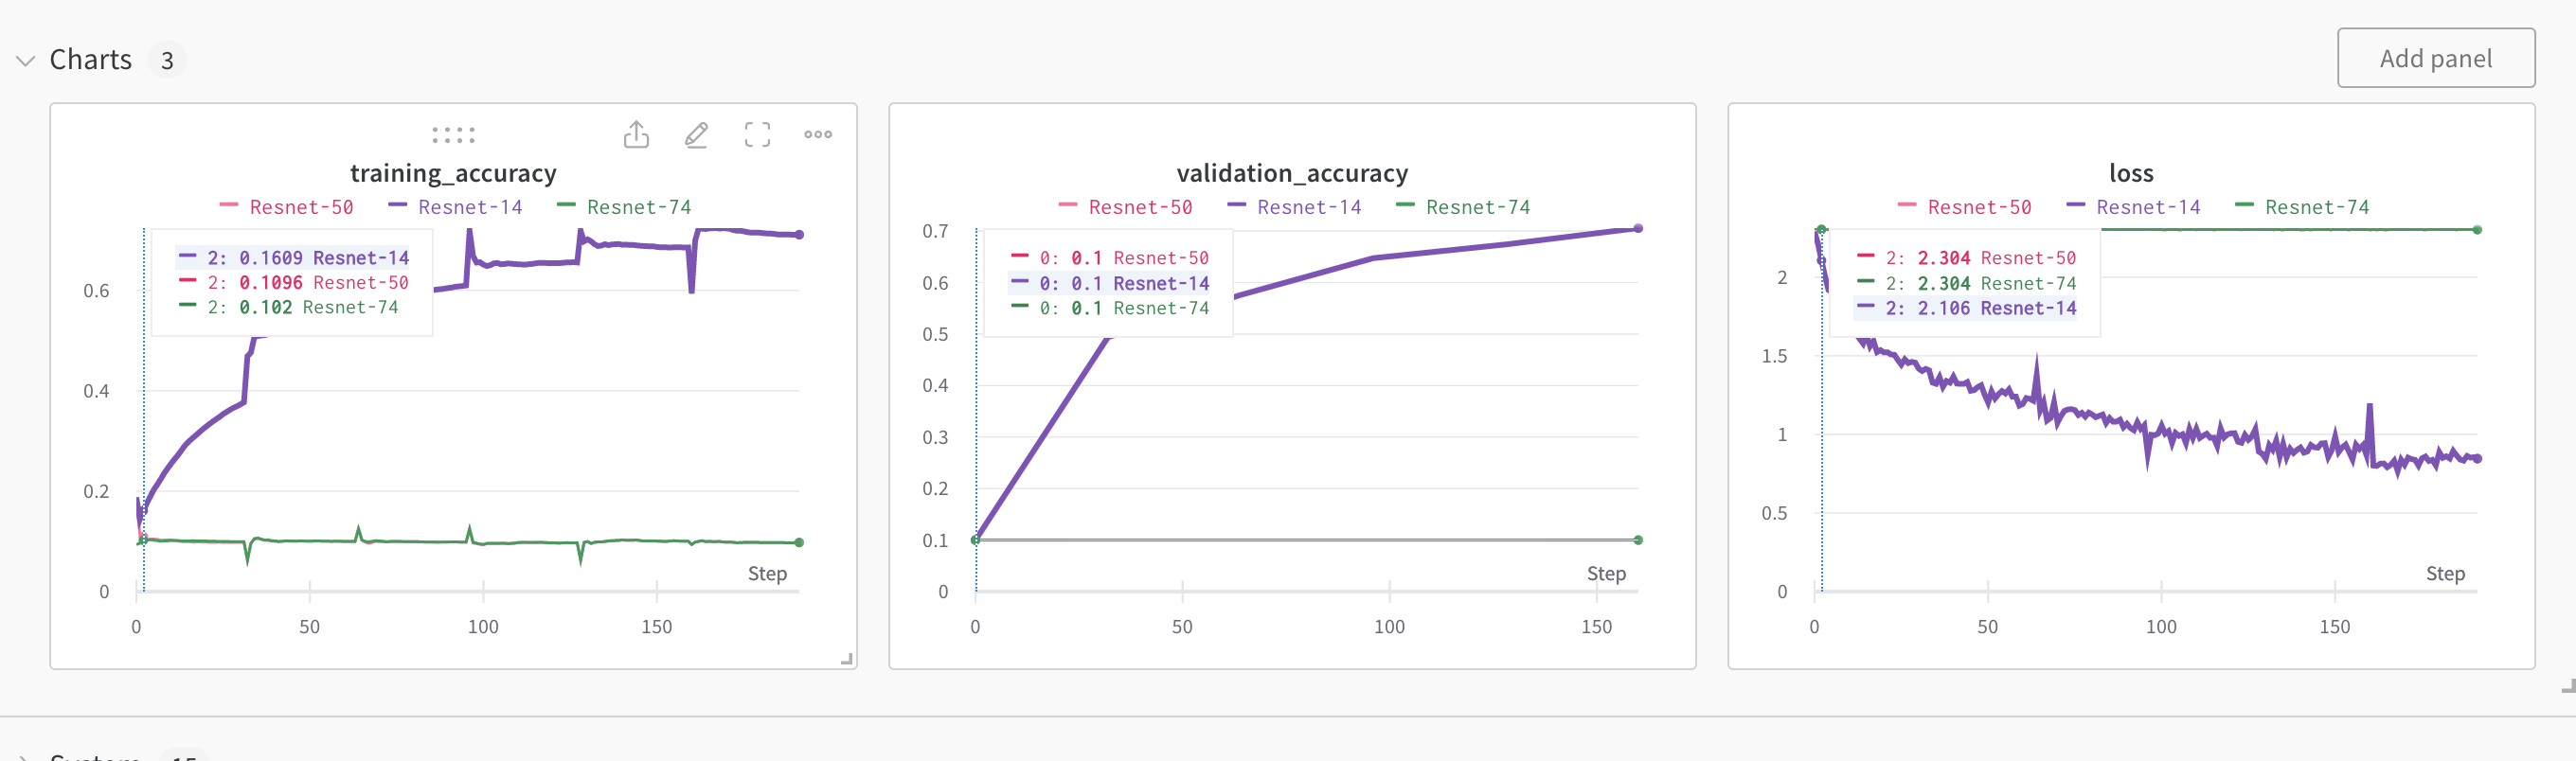
\includegraphics[width=240pt,height=100pt]{./img/result}
    \caption{Résultats des modèles ResNet sur le jeu de données CIFAR-10}\label{fig:result}
\end{figure}

Nous constatons que les trois modèles ont une précision élevée sur le jeu de données CIFAR-10.
La précision augmente avec la profondeur du réseau. ResNet-50 est le modèle qui obtient la meilleure performance,
avec une précision de 94,1\% sur l'ensemble de test.

\section{Analyse critique de l'approche}

L'utilisation du jeu de données CIFAR-10 est un bon choix pour tester la performance des modèles de ResNet,
car il s'agit d'un jeu de données standard pour la reconnaissance d'images et il est assez complexe pour évaluer
la performance des modèles.
Cependant, le choix d'un jeu de données de taille plus importante pourrait permettre d'évaluer la performance
des modèles à une plus grande échelle.
a durée de l'entraînement de 10 époques semble raisonnable pour le jeu de données CIFAR-10 et pour les
modèles de ResNet testés. Il serait intéressant d'explorer l'impact de la durée de l'entraînement sur la
performance des modèles et de trouver un juste équilibre entre la performance et la durée d'entraînement.

\section{Conclusion}

Ce projet a permis d'explorer des performances des réseaux de neurones profonds pour la classification d'images,
en se concentrant sur les modèles ResNet qui ont été introduits pour surmonter les problèmes de dégradation de
performances rencontrés par les réseaux profonds traditionnels.
Les résultats obtenus ont confirmé l'efficacité des modèles ResNet pour la reconnaissance d'images, en montrant
que les modèles de ResNet profonds (ResNet-34 et ResNet-50) ont atteint des performances de classification élevées
sur le jeu de données CIFAR-10.
Depuis leur introduction en 2016, les modèles ResNet ont été largement utilisés dans divers domaines, notamment
la reconnaissance d'images, la segmentation d'images, la détection d'objets et la classification de textes.
Les modèles utilisant ResNet pour différentes tâches: ResNeXt, Wide ResNet, YOLO, GANs, etc.

\bibliographystyle{named}
\bibliography{rapport}

\end{document}
